\section{Ergebnisse}
\label{sec:ergebnisse}

\subsection{Durchlaufzeiten}

\begin{table}[htbp]
  \centering
  \caption{Mittlere Durchlaufzeiten je Stufe ($n=30$).}
  \label{tab:zeiten}
  \begin{tabular}{l S[table-format=2.2] S[table-format=2.1]}
    \toprule
    Stufe & {Mittelwert (\si{\second})} & {Anteil (\%)} \\
    \midrule
    Bearbeiten     & 0,00 &  0,0 \\
    Kompilieren    & 2,41 & 58,7 \\
    Auswerten      & 1,09 & 26,5 \\
    Veröffentlichen& 0,61 & 14,8 \\
    \bottomrule
    Summe          & 4,11 & 100,0 \\
  \end{tabular}
\end{table}

Wie \cref{tab:zeiten} zeigt, dominiert die Kompilierung die Gesamtdauer.
\cref{fig:anteile} veranschaulicht die Verteilung.

\begin{figure}[htbp]
  \centering
  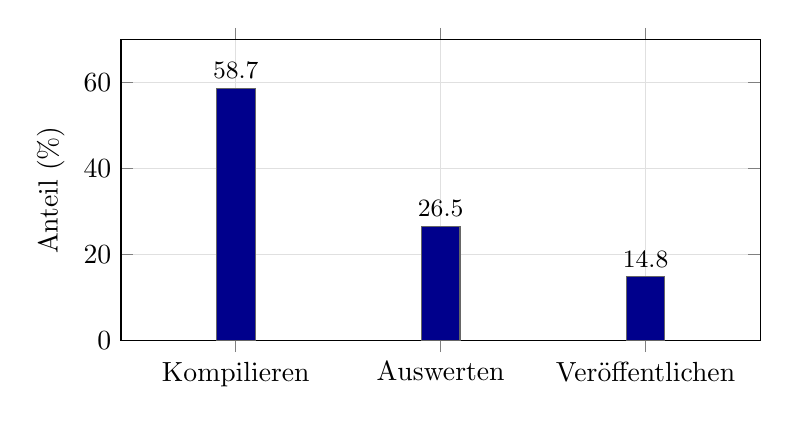
\begin{tikzpicture}
    \begin{axis}[
        ybar,
        width=0.8\linewidth,
        height=5.4cm,
        bar width=14pt,
        symbolic x coords={Kompilieren, Auswerten, Veröffentlichen},
        xtick=data,
        ylabel={Anteil (\%)},
        ymin=0, ymax=70,
        nodes near coords,
        nodes near coords align={vertical},
        every node near coord/.append style={font=\small},
        grid=major,
        grid style={black!12},
        enlarge x limits=0.28,
      ]
      \addplot[fill=blue!55!black, draw=black!60] coordinates {
        (Kompilieren,58.7) (Auswerten,26.5) (Veröffentlichen,14.8)
      };
    \end{axis}
  \end{tikzpicture}
  \caption{Anteile der Stufen an der Gesamtdauer.}
  \label{fig:anteile}
\end{figure}

\subsection{Fehlerquote}

Über alle Läufe traten vier Fehler auf: dreimal eine fehlerhafte Gleichungs-
nummerierung, einmal eine nicht aufgelöste Literaturreferenz. Die Fehlerquote
beträgt damit
\[
  f \;=\; \frac{4}{30} \cdot 100\,\% \;\approx\; 13{,}3\,\%.
\]

\subsection{Diskussion}
\label{sec:diskussion}

\begin{itemize}[leftmargin=*]
  \item Der hohe Anteil der Kompilierung spricht für Auto-Build mit
    Verzögerung statt Bauen bei jedem Tastendruck.
  \item Die Auswertung lässt sich parallelisieren; der Gewinn ist in
    \cref{tab:zeiten} noch nicht enthalten.
  \item Nicht aufgelöste Verweise werden von \emph{LaTeX Studio} direkt in der
    Problemliste angezeigt und per Klick geöffnet.
\end{itemize}

\begin{hinweis}{Automatische Problemerkennung}
  Wechseln Sie nach einem fehlgeschlagenen Build in das Register
  \emph{Probleme} im unteren Bereich -- jede Zeile führt zur betreffenden
  Stelle im Quelltext.
\end{hinweis}
